\section{Probability}
\paragraph{Definitions:}
\begin{itemize}
	\item Probability: Proportion of an outcome in the long run \textcolor{Gray}{(Converges due to law of large numbers)}
	\item Sample Space: Set of ALL possible outcomes
	\item Event: A particular outcome, OR Set of possible outcomes (event $\subseteq$ Sample space)\\
		$P(Event)=\sum P(Outcome)$
	\item Disjoint Events $A,B\iff A\cap B = \varnothing$
	\item Independent Events $A,B$
		\begin{align*}
			&P(A\cap B)&=P(A)\times P(B)\\
			&P(A|B)&=P(A)\\
			&P(B|A)&=P(B)
		\end{align*}
\paragraph{Probability Cheatsheet}
\begin{align*}
	P(A\cup B)&=P(A)+P(B)\\
			  &\quad-P(A\cap B)\\
			  &=P(A)+P(B) \textup{(Disjoint)}\\
	P(A\cap B)&=P(A)\times P(B|A)\\
			  &=P(B)\times P(A|B)\\
			  &=P(A)\times P(B)\textup{(Independent)}\\
	P(A\cap B\cap C)&=P(A)+P(B)+P(C)\\
					&\quad-P(A\cap B)-P(A\cap C)\\
					&\quad-P(B\cap C)-\\
					&\quad P(A\cap B\cap C)\\
	P(A|B)&=\frac{P(A\cap B)}{P(B)}\\
		  &=P(A)\times \frac{P(B|A)}{P(B)}
\end{align*}
For $B_i,B_2,...,B_n$ partitioning S\\
\begin{align*}
	P(A)&=\sum_{i=1}^nP(A\cap B_i)\\
	    &=\sum_{i=1}^n\{P(A|B_i)P(B_i)\}
\end{align*}
\begin{Figure}
	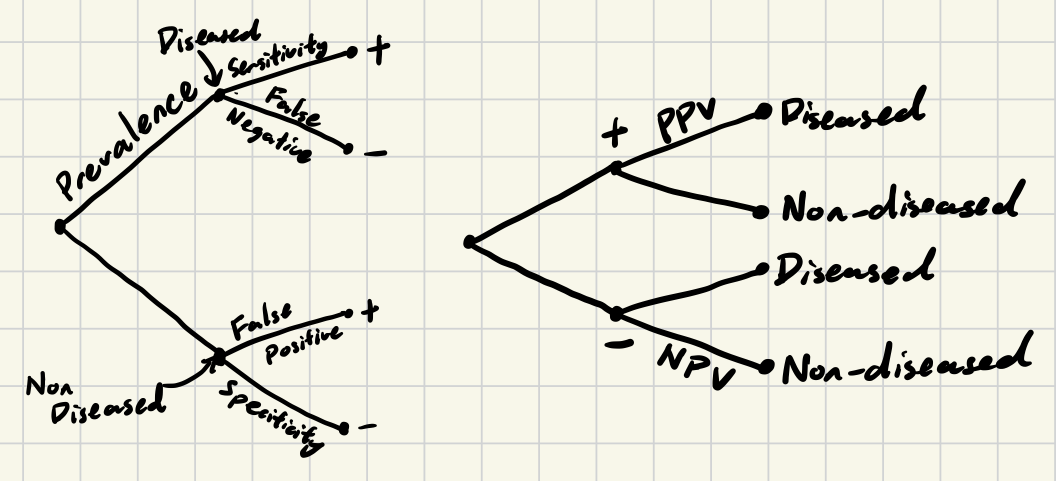
\includegraphics[width=0.893\linewidth]{diseaseProbabilities.png}
\end{Figure}
\end{itemize}